\documentclass[A4paper]{gdv/gdv}

\usepackage{epic}
\usepackage{eepic}
\usepackage{amssymb,amsmath}
\usepackage{version}
\usepackage{url}
\usepackage[utf8]{inputenc}
\usepackage[margin=10pt,labelfont=bf]{caption}
\usepackage{graphicx}
\usepackage{hyperref}
\usepackage{csquotes}

\newcommand{\til}{\raise.17ex\hbox{$\scriptstyle\sim$}}	% http://stackoverflow.com/questions/256457/how-does-one-insert-a-backslash-or-a-tilde-into-latex

\newcommand{\todo}[1]{\textbf{Todo:\ #1}}
\newcommand{\note}{\textit{Note:}\ }
\newcommand{\teilaufgabe}[1]{\textbf{#1.}}

\begin{document}
\begin{gdvSheet}

% hier müssen whitespaces hin!

\kopf{Daniel Langbein, Ediz Kocak, Hisham Görner, Michelle Bastian}{17.01.2022}{GraPRA: Graphics Programming and Application}{5}


\newcommand{\file}[1]{\texttt{#1}}
\newcommand{\code}[1]{\texttt{#1}}

%########################################################################################

\textbf{The island of two faces.}
In a cooperative multiplayer, the players build and craft items during the day to prepare themselves for the dark nights where they are attacked by dangerous creatures.
One can either craft weapons by mining different types of blocks and combining them or by picking up weapons of dead creatures in the night.

\textbf{Abgabe bis 09.02.2022, Mitternacht.}
\textbf{Präsentation am 11.02.2022, vorläufig 10:00}

\vspace*{32px}

\begin{figure}[ht]
	\centering
	
\includegraphics[width=.7\textwidth]{img/water}
	\caption{Water reflections. \href{https://www.reddit.com/r/Optifine/comments/krr89r/minecraft_can_be_beautiful_with_the_right_shaders/}{Source}.}\label{fig:water}
\end{figure}

\vspace*{12px}

\underline{\aufgabe{1--6}{8}{Graphical Effects}}

The first 5 numbers describe the graphical effects.
Before you can start with them, roughly read through numbers 7--10 and set up a basic rendering pipeline.

\aufgabe{1}{2}{Water}
$[$Hisham$]$

\teilaufgabe{Reflections}
Create water that reflects the scene depending on the view angle.
Render the scene from under the water and blend with water texture.
See figure~[\ref{fig:water}].

\teilaufgabe{Refraction}
Mimic the way light bends when passing from air into water.

\teilaufgabe{Normal maps + specular highlighting}
Simulate water movement and highlight bright reflection spots.
See figure~[\ref{fig:sun}].

\aufgabe{2}{1}{Day-night-cycle}
$[$Daniel$]$

\begin{figure}[ht]
	\centering
	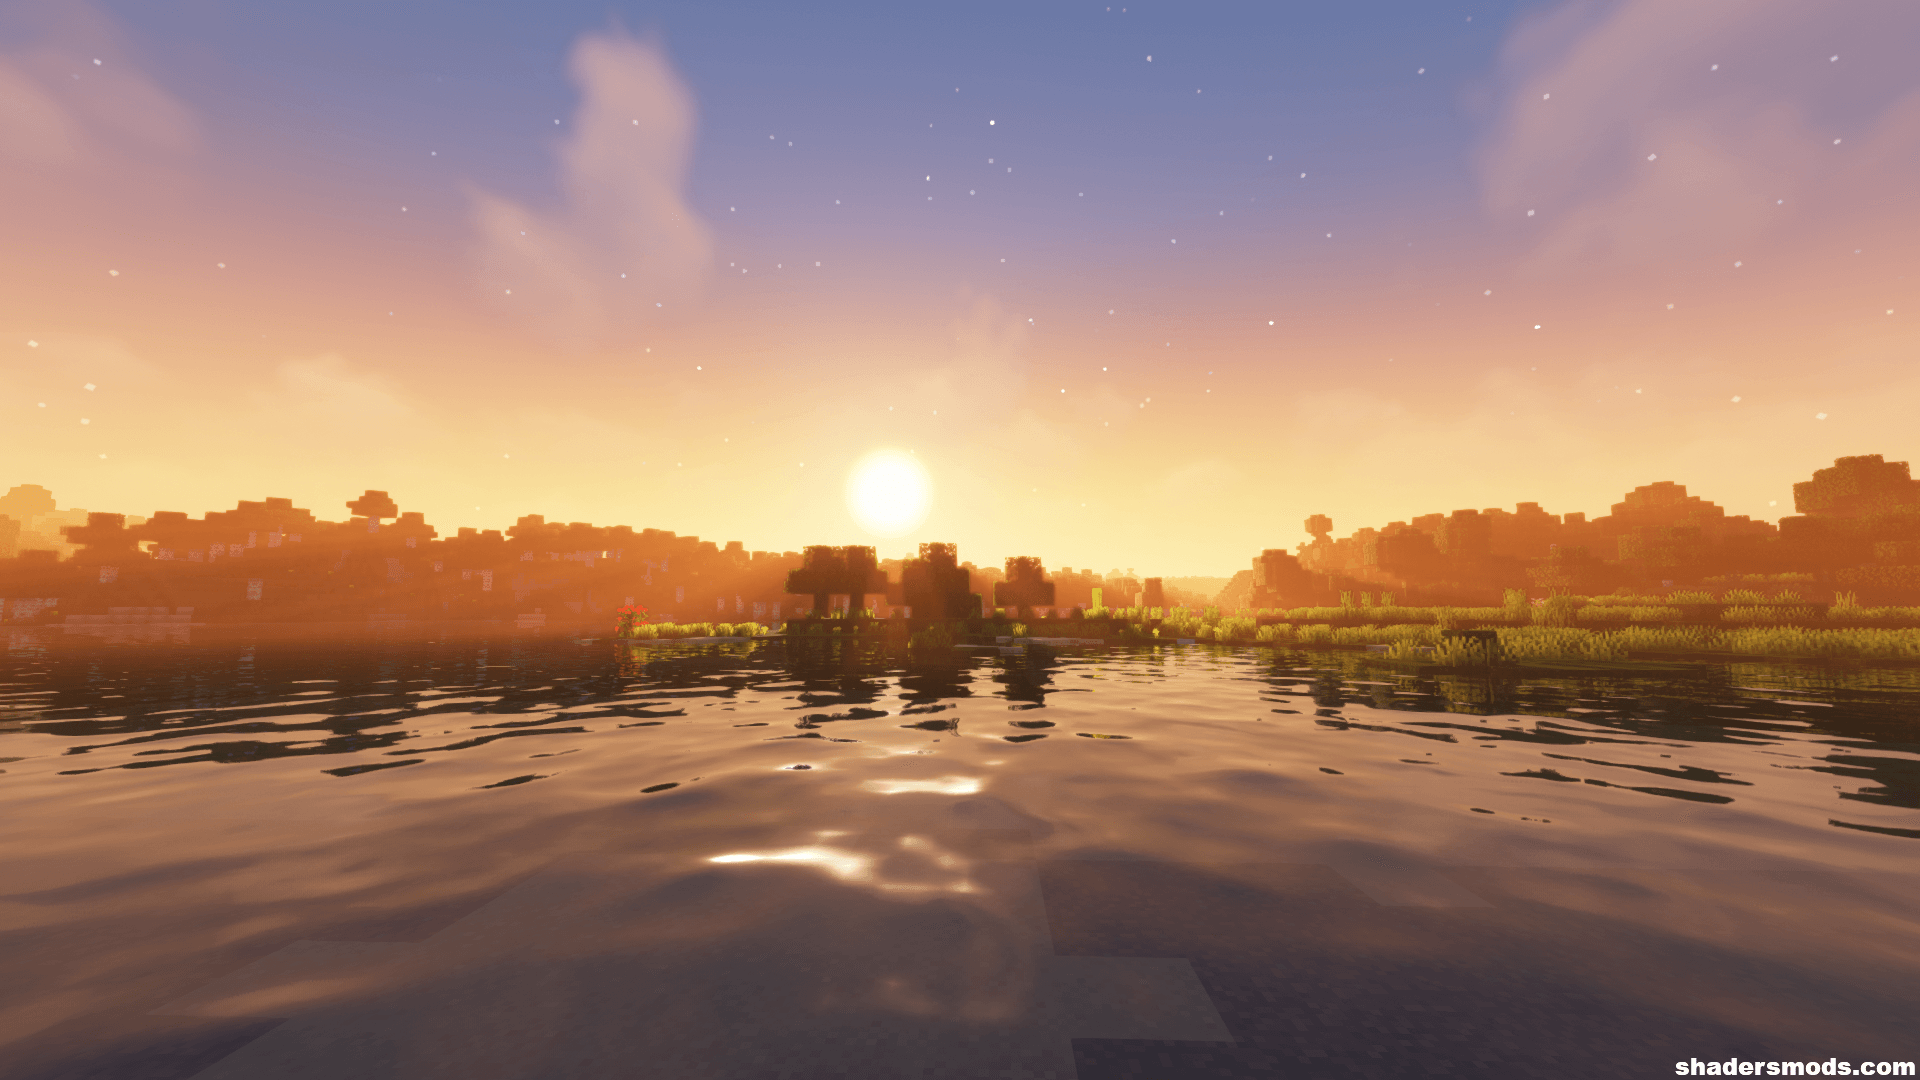
\includegraphics[width=.4\textwidth]{img/sunset}
	\caption{Sunset. \href{https://shadersmods.com/complementary-shaders/}{Source}.}\label{fig:sun}
\end{figure}

\teilaufgabe{Atmosphere}
Add a sky-sphere with separate models for the sun and moon.
The shadows should depend on the current position of the sun/moon.
Also add a day-night-cycle with sunset and sunrise that impacts the color temperature.
See figure~[\ref{fig:sun}].

\aufgabe{3}{2}{Light sources}
$[$Daniel, Hisham$]$

\begin{figure}[ht]
	\centering
	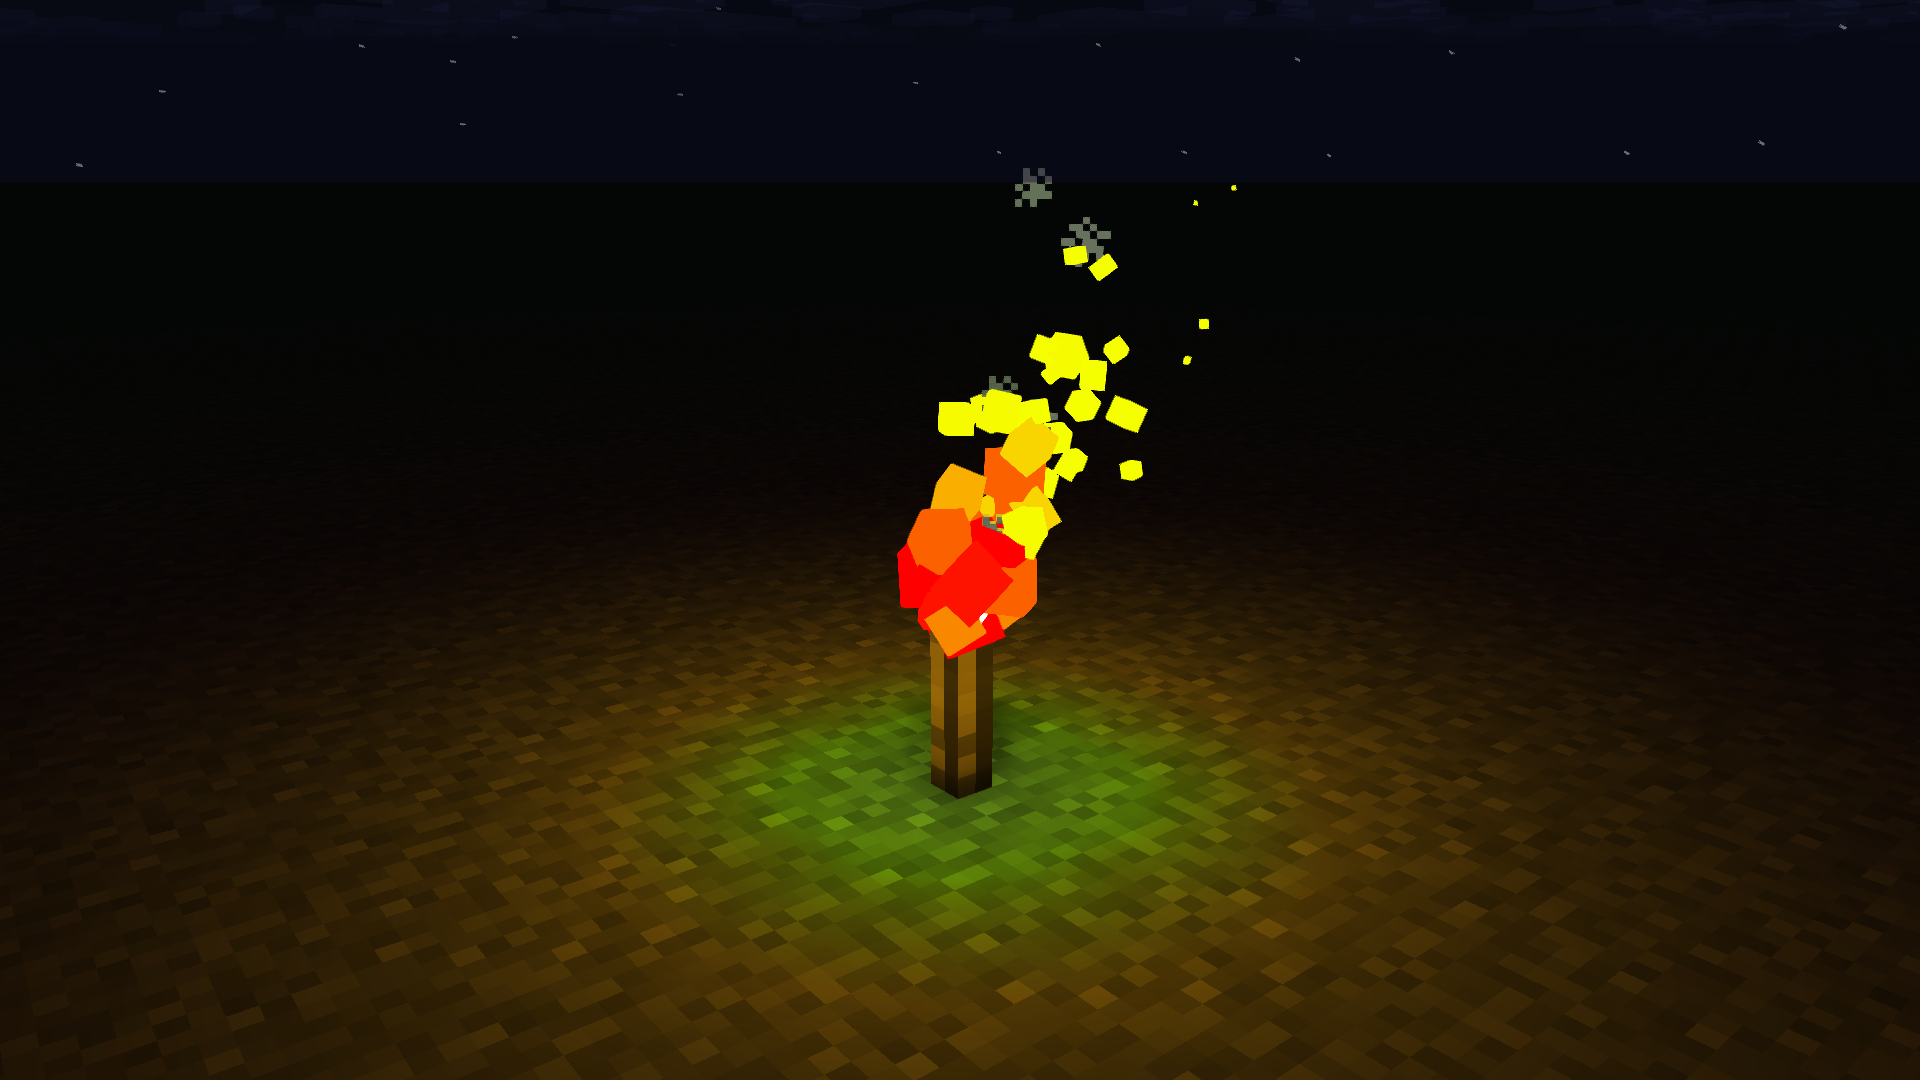
\includegraphics[width=.4\textwidth]{img/torch}
	\caption{Torch. \href{https://www.mineimatorforums.com/index.php?/topic/62414-advanced-torch-rig/}{Source}.}\label{fig:torch}
\end{figure}

\teilaufgabe{Torches}
Add torches that emit point lights and particles.
See figure~[\ref{fig:torch}].

\teilaufgabe{Shadows}
Basic and point shadows.

\aufgabe{4}{2.5}{Weather effects}
$[$Ediz, Michelle$]$

\begin{figure}[ht]
	\centering
	
\includegraphics[width=.4\textwidth]{img/rain}
	\caption{Rain. \href{https://www.reddit.com/r/Optifine/comments/kiifzm/bsl_shaders_rain_reflection_not_working/}{Source}.}\label{fig:rain}
\end{figure}

\begin{figure}[ht]
	\centering
	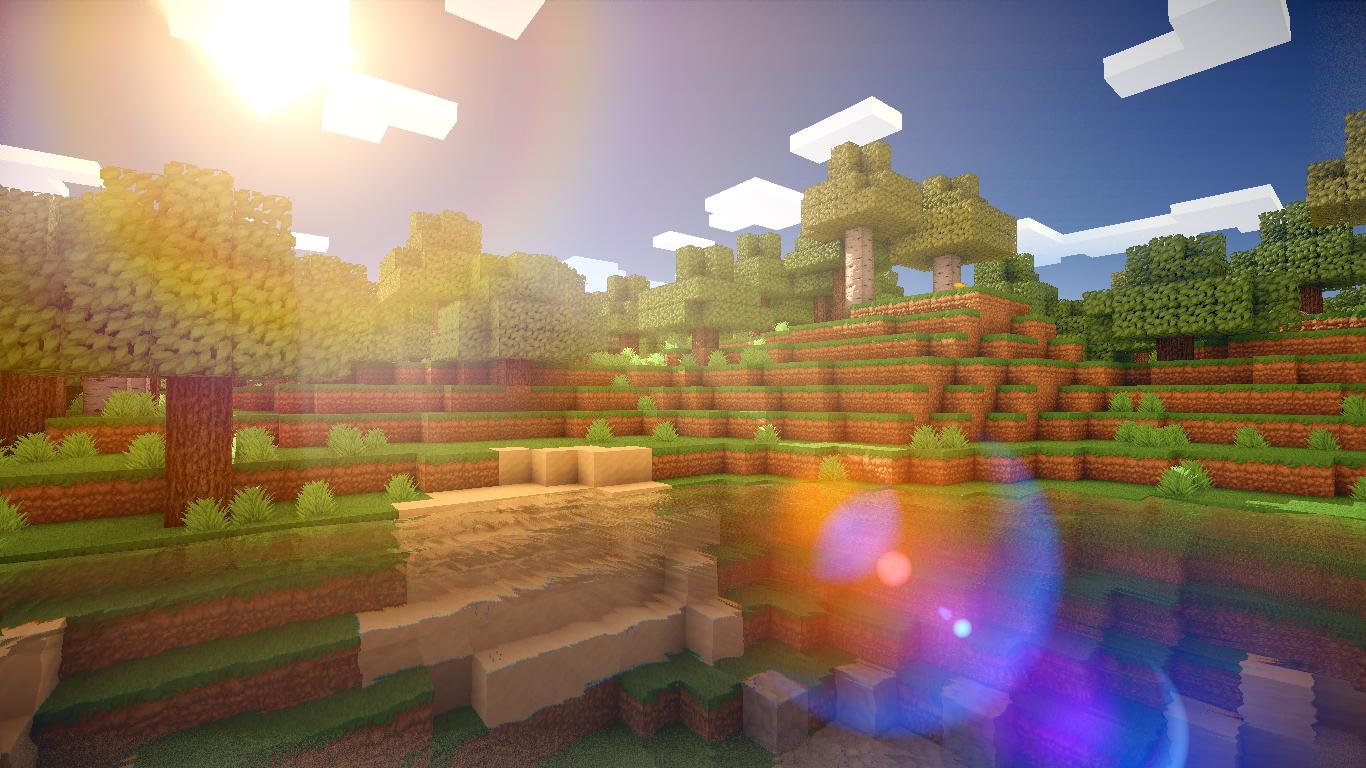
\includegraphics[width=.4\textwidth]{img/lens-flare}
	\caption{Lens-flare. \href{https://www.minecraftforum.net/forums/mapping-and-modding-java-edition/minecraft-mods/1293898-1-14-chocapic13s-shaders?page=2}{Source}.}\label{fig:flare}
\end{figure}

\teilaufgabe{Lens-flare}
Replicate lens-flare by drawing sprites along light ray, taking placement, brightness, blur and occlusion int account.
See figure~[\ref{fig:flare}].

\teilaufgabe{(Block-)clouds}
Add simple, solid clouds.

\teilaufgabe{Rain}
Set Atmosphere by darkening clouds and the overall scene.
Limit view size, add rain and a thunderstruck that lightens the scene, hits the ground and draws shadows.
See figure~[\ref{fig:rain}].

\aufgabe{5}{0.5}{Screen effects}
$[$Ediz, Michelle$]$

\teilaufgabe{Zoom}
Slight zoom-in when the player runs.

\teilaufgabe{Hit effect}
Slightly red tint on the players screen when being hit.

\begin{figure}[ht]
	\centering
	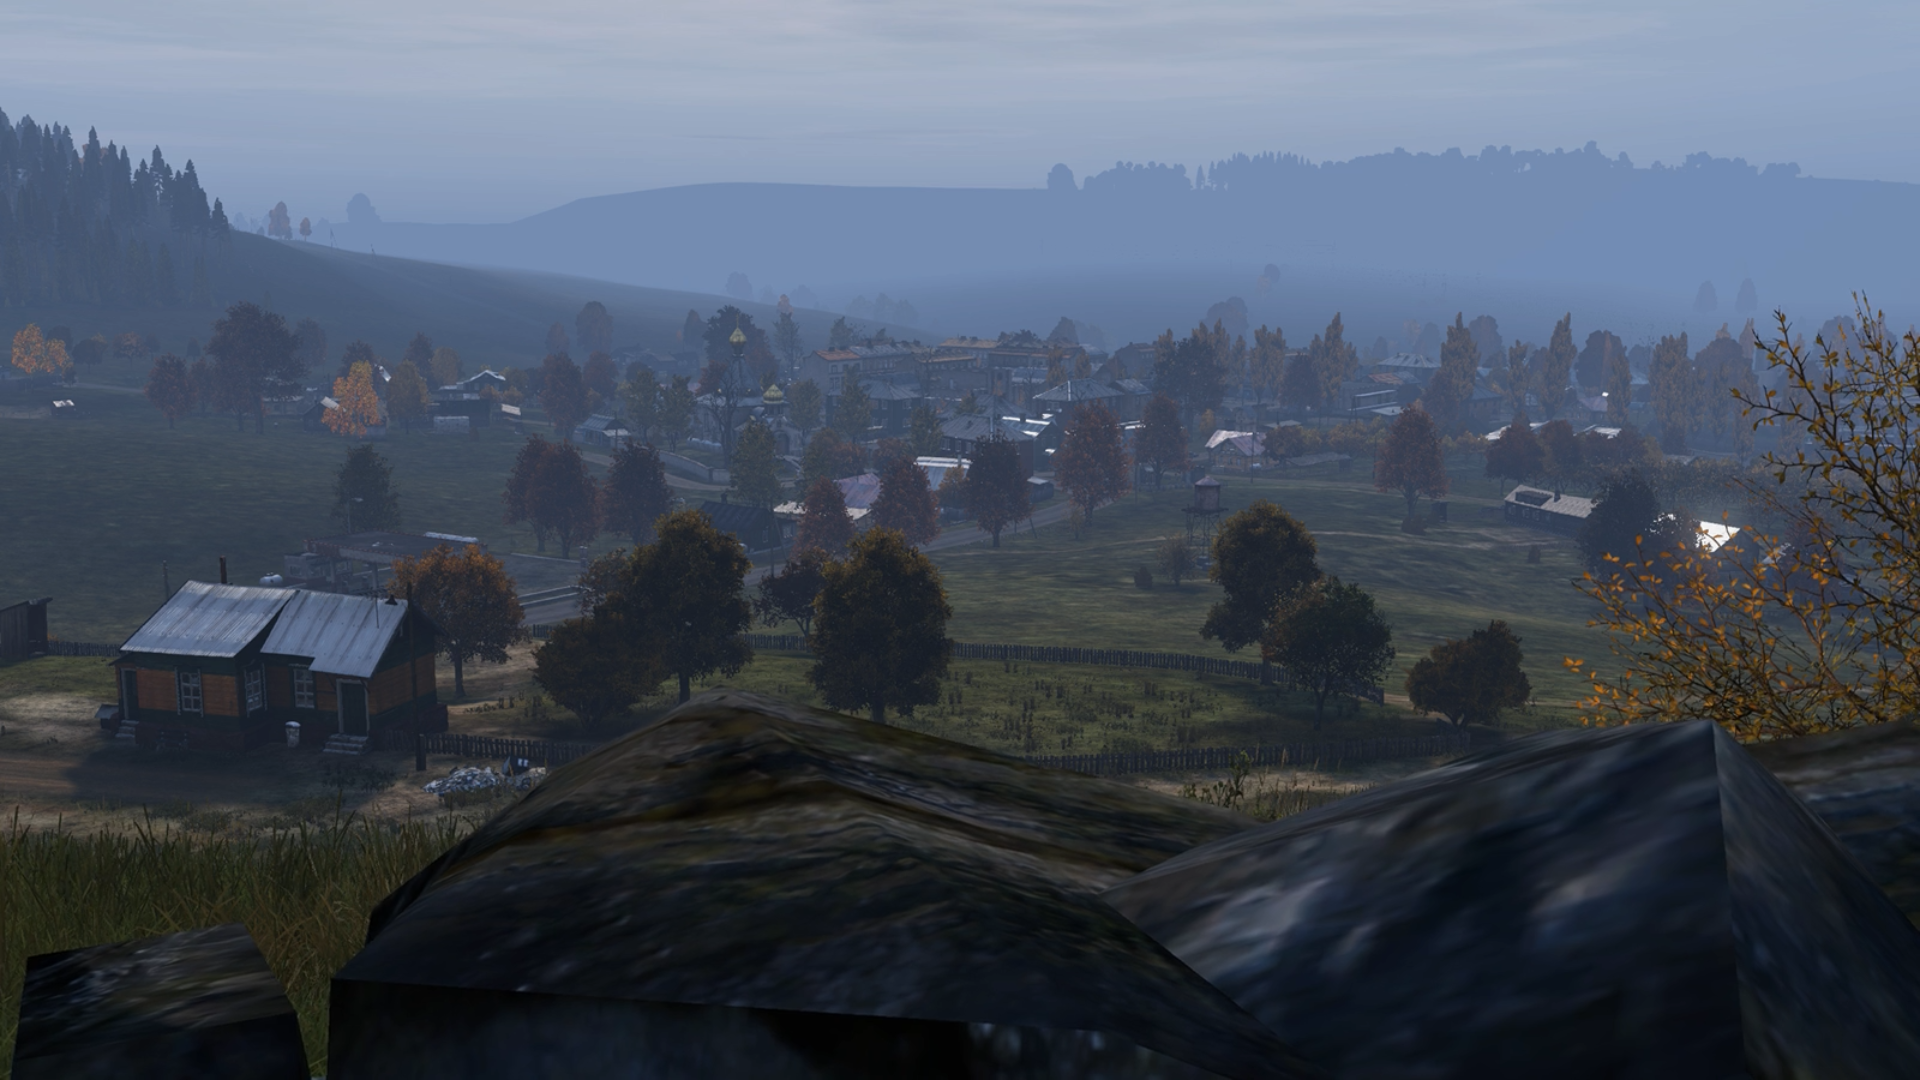
\includegraphics[width=.4\textwidth]{img/distance-blue}
	\caption{Aerial perspective. \href{https://feedback.bistudio.com/T141632}{Source}.}\label{fig:blue}
\end{figure}

\teilaufgabe{Aerial perspective}
Imitate Rayleigh-scattering in distance by reducing color values and giving them a blue tint.
See figure~[\ref{fig:blue}].



\pagebreak
\underline{\aufgabe{6--10}{10}{Game play}}

The last 5 numbers are all about the gameplay.

\aufgabe{6}{3}{Multiplayer}
$[$Daniel, Hisham$]$

Implement a client-server architecture to allow multiple players join the same cooperative game.
Take care of synchronizing the map state:

\begin{itemize}
	\item If two players dig the same block simultaneously, only one should get the item.
	\item Animations and moving objects (e.g.\ projectiles) should be in sync on each player's screen.
\end{itemize}

\aufgabe{7}{2}{Basic features}
$[$Daniel, Ediz, Hisham, Michelle$]$

\teilaufgabe{Design}
A scene with an island surrounded by water and self modeled meshes: 2 enemies (one zombie running at players, one skeleton throwing a projectiles), flowers, trees, grass, items (sword, axe, torch).
GUI related implementations: Menu, player inventory (half-transparent when inactive).

\teilaufgabe{Movement}
First person Camera with a marker (e.g.\ cross) in the center of the screen.
Smooth player and NPC movement with skeleton-animations (when walking, mining, attacking or throwing projectiles).

\teilaufgabe{Crafting}
A player can change the terrain by mining and placing blocks.
Highlight the block in the center-front of the player (if not too far away).
Show a progress cycle and particles when mining a block.
Mined blocks are collected in the players inventory.
If a player has the required blocks in its inventory, it can craft weapons and torches.

\aufgabe{8}{2}{Cooperative Gameplay}
$[$Ediz, Michelle$]$

At the beginning, the players spawn at random positions across the island during daytime.
The first task is to find each other and prepare for the night.
During the day there are animals (dog, horse) walking around.

The players should prepare for the night to be able to defend themselves from enemies.
After dawn enemies spawn in dark spots and start attacking the players with various weapons.
(Some) enemies drop their weapons when they die and the players can pick those up.

When a player is hit (by weapon or projectile), it looses health-points (HP).
HP do only regenerate during daytime.
If a player died, it spawns at some random position in some distance to the other alive players.
That player can't move until 30s have passed and the other alive players are close to it to \enquote{free} it.

The game is lost if all players are dead or not free at the same time.

\aufgabe{9}{2}{Fighting}
$[$Ediz, Michelle$]$

Model and animate at least two hand-weapons that can be crafted:

\begin{itemize}
	\item A sword is fast to swing and makes not the most damage.
		  But it is well suited to block attacks of enemies.
	\item An axe that has more impact but is slower.
\end{itemize}

There should also be at least one projectile type that is thrown by some enemies which can be picked up and thrown back (but not crafted).
Projectiles are great for long-distance fighting.

Implement some logic to detect collisions of players and enemies with projectiles adding damage to them.
Also detect blows from hand weapons.

\aufgabe{10}{1}{Sound}
$[$Daniel, Ediz, Michelle$]$

Auditory enhancement through different sounds when walking on surfaces, rain, thunderstruck and overall soundtrack (different mood during peaceful day and dangerous night).
Distant sounds (e.g.\ by other walking players) should be quieter and localized.

\vspace*{30px}

% \pagebreak
% \bibliographystyle{plain}
% \bibliography{lit}

\vfill\hfill Happy Hacking!~:) \hfill\ %\vfill

\end{gdvSheet}

\end{document}
